% Werke X/1 (1917), native167–169, printed160–162.
\begingroup
\setlength{\headheight}{25pt}
\SourceLeaf{167}\NoSourceHead
\SourceGroup{III}
\HistoricTitle{[TEILUNG DER LEMNISKATE.]}
\HistoricCitation{[Eintragungen im \textsc{Leiste}.]}
\NumberedItem{1}
\noindent{\small [S. 69]}
\par\indent Die Theilung der Lemniscata in sieben Theile gibt die Gleichung:
\[16(1-x^4)\left(\begin{array}{rrrrr}1&-5&-5&+1&\\\hline1&+20&-26&+20&+1\end{array}\right)^2
=\left(\begin{array}{rrrrr}3&\ast&-6&\ast&-1\\\hline1&\ast&+6&\ast&-3\end{array}\right)^2.\]
\NumberedItem{2}
\noindent{\small [S. 87]}
\par\indent Sit \(\sin\tfrac15kR=(k)\), tum habebuntur aequationis radices \((0),\ \pm(4),\ \pm(2),\)
\par\medskip
\noindent\begin{minipage}{.55\linewidth}
\[\begin{gathered}
\frac{(0)+(5)(4)(1)\surd-1}{(1)-(0)(5)\ldots}\\[9pt]
\frac{(4)+(1)(4)(1)\surd-1}{(1)-(4)(4)(1)\surd-1}\\[9pt]
\frac{(2)-(3)(4)(1)\surd-1}{(1)+(2)(3)(4)\surd-1}
\end{gathered}\]
\end{minipage}\hfill\begin{minipage}{.4\linewidth}
\centering
\begin{tikzpicture}[x=1cm,y=1cm,line width=.65pt]
\draw (0,0) .. controls (-.7,.6) and (-1.45,.9) .. (-1.8,.35)
 .. controls (-2.3,-.45) and (-.9,-.8) .. (0,0)
 .. controls (.75,.6) and (1.6,.85) .. (1.85,.25)
 .. controls (2.15,-.5) and (.9,-.9) .. (0,0);
\draw (-1.03,.40)--(-.92,.69);
\draw (-1.56,-.62)--(-1.40,-.33);
\draw (1.39,.34)--(1.50,.63);
\draw (.88,-.66)--(1.02,-.37);
\end{tikzpicture}
\end{minipage}
\[\renewcommand{\arraystretch}{1.5}\begin{array}{lc|}
\pm1,\ \surd-1\left[\begin{array}{c}\frac{(0)}{(2)}\\(4)\end{array}\right|&
\dfrac{(4)}{(1)}.\dfrac{1+(1)(1)\surd-1}{1-(4)(4)\surd-1}\\[6pt]
&\dfrac{(2)}{(3)}\ \dfrac{1+(3)(3)\surd-1}{1-(2)(2)\surd-1}
\end{array}\]
\clearpage
\SourceLeaf{168}\fancyhead{}\fancyhead[R]{\small161}\fancyhead[C]{\scriptsize\shortstack{ÄLTESTE UNTERSUCHUNGEN ÜBER\\ LEMNISKATISCHE FUNKTIONEN.\quad III.}}
\NumberedItem{3}
\noindent{\small [S. 90--91]}
\par\medskip
\begingroup\small\setlength{\arraycolsep}{3pt}
\noindent\begin{minipage}[b]{.38\linewidth}
\[\renewcommand{\arraystretch}{1.8}\begin{array}{rrl}
1&1{,}31102877&\left[=\frac{\varpi}{2}\right]\\
2&1{,}71879545&\\4&2{,}95416&\\5&3{,}87311&\\6&5{,}07777&\\8&8{,}72765&\\9&11{,}44320&\\10&15{,}00&
\end{array}\]
\end{minipage}\hfill\begin{minipage}[b]{.58\linewidth}
\[\renewcommand{\arraystretch}{1.5}\begin{array}{rrl}
\multicolumn{3}{l}{[\cos18^0]}\\
&0{,}965425785&[=\mu18^0]\\
&1{,}034180311&[=\nu18^0]\\[5pt]
\multicolumn{3}{l}{\sin36^0}\\
&0{,}524411511&\left[=\frac{\varpi}{5}\right]\\
-&661011&\\-&292&\\\cline{1-2}
&0{,}523750208&[=M36^0]\\
&1{,}006302208&\left[=1+\frac1{12}\left(\frac{\varpi}{5}\right)^4\right]\\
-&567&\\\cline{1-2}
&[1{,}006301641&=N36^0]
\end{array}\]
\end{minipage}
\endgroup
\[\begin{aligned}
[\sin]\,36^0&=\\[-2pt]
&\frac{0{,}523750208}{1{,}006301641}=0{,}5204703904.\\[12pt]
[\sin]\,72^0&=\cos18^0\\[-2pt]
&\frac{0{,}965425785}{1{,}034180311}=0{,}9335177577.
\end{aligned}\]
\NumberedItem{4}
\noindent{\small [S. 102]}
\par\indent Die Theilung der Lemniscata in 5 Theile führt auf diese Gleichung
\[\frac{9-36x^4+30x^8+12x^{12}+x^{16}}{1+12x^4+30x^8-36x^{12}+9x^{16}}=\frac{4(1-x^4)}{1+2x^4+x^8}\]
\[\left.\renewcommand{\arraystretch}{1.35}\begin{array}{rrrrrrr}
9&-36&+30&+12&+1&&\\
&+18&-72&+60&+24&+2&\\
&&+9&-36&+30&+12&+1\\
-4&-48&-120&+144&-36&&\\
&+4&+48&+120&-144&+36&\\\hline
5&-62&-105&+300&-125&+50&+1
\end{array}\right\}=0.\]
\par\noindent{\small X1.}\hfill{\small21}
\clearpage
\SourceLeaf{169}\ArithmeticHead{162}{L}{ANALYSIS.\quad NACHLASS.}
\noindent[Wurzeln dieser Gleichung vom 24. Grade sind \(\sin\text{ lemn }\frac{k\varpi}{5}\) für \(k=1,2,3,4\), die übrigen sind imaginär, also:]
\begin{center}\textit{Determ. rad. imag.}\end{center}
\[\frac{\square}{\square}=\frac{4(1-x^4)}{\square},\]
\noindent[setze \(x^4=y\), so ist]
\[(3-6y-yy)(1+y)=2(1+6y-3yy)\surd(1-y)\]
\[\begin{gathered}
S=\surd720-26\ [=12\surd5-26]\\[5pt]
\left[=\left(\sin\text{ lemn }\frac{2\varpi}{5}\right)^4+\left(\sin\text{ lemn }\frac{4\varpi}{5}\right)^4\right]
\end{gathered}\]
{\small\[\begin{array}{rl}
349-156\surd5&\\
-9+\phantom{15}4\surd5&\\\cline{1-1}
340-152\surd5&\left[=\frac12\left(\sin\text{ lemn }\frac{4\varpi}{5}\right)^4-\frac12\left(\sin\text{ lemn }\frac{2\varpi}{5}\right)^4\right]^2.
\end{array}\]}
\noindent Zwei Wurzeln obiger Gleichung sind
\[\begin{aligned}
&+0{,}0733810047\ \left[=\left(\sin\text{ lemn }\frac{2\varpi}{5}\right)^4\right]\\
&+0{,}7594355\ \left[=\left(\sin\text{ lemn }\frac{4\varpi}{5}\right)^4\right].
\end{aligned}\]
\NumberedItem{5}
\noindent{\small [S. 100--101]}
\par\indent Auflösung der Gleichung
\[5-62x-105xx+300x^3-125x^4+50x^5+x^6\ [=0^{*)}]\]
\noindent[Es folgt eine Zahlenrechnung, anscheinend nach der Regula falsi].
\par\indent Also eine Wurzel
\[=0{,}07338100477\ \left[=\left(\sin\text{ lemn }\frac{2\varpi}{5}\right)^4\right]\]
\noindent und folglich
\[\sin36^0=0{,}52047024\ [={}^4\!\surd0{,}073381].\]
\renewcommand{\thefootnote}{[*)}\footnotetext{Das \(x\) in dieser Gleichung ist die vierte Potenz der im art. [4.] ebenso bezeichneten Unbekannten; die Gleichung hat also die Wurzeln \(\left(\sin\text{ lemn }\frac{k\varpi}{5}\right)^4\) für \(k=1,2,3,4\).]}
\clearpage
\endgroup
